\documentclass[11pt]{article}

% Pacotes
\RequirePackage{luatex85}
\usepackage{amsmath}
\usepackage{amssymb}
\usepackage{graphicx}
\usepackage[colorlinks=true, allcolors=blue]{hyperref}
\usepackage{amsthm}
\usepackage{framed, color,xcolor}
\usepackage{stmaryrd}
\usepackage{rotating}           % Usado para rotacionar o texto
\usepackage[all,knot,arc,import,poly]{xy}   % Pacote para desenhos gráficos
% Este pacote pode conflitar com outros pacotes gráficos como o ``pictex''
% Então é necessário usar apenas um dos pacotes conflitantes
\usepackage{tikz, tikz-cd}
\usepackage{epigraph}
\usetikzlibrary{babel}
\usetikzlibrary{positioning}
\usetikzlibrary{calc}
\usepackage[stix2]{newtxmath}
\usepackage{mathtools, nccmath}
%\usepackage[usenames,dvipsnames]{xcolor}
\usepackage{amssymb, mathrsfs}
\usepackage[numbers]{natbib}
\usepackage{fontspec}
\usepackage{enumitem} % pra substituir o símbolo do itemize por alguma coisa legal, tipo setinhas:  \begin{itemize}[label=\ding{212}]
\usepackage{pifont}
\usepackage{stmaryrd} % for \arrownot (notação de adjacência em grafo)
\usepackage{quiver} %pacote do quiver pra desenhar diagramas mais legais

%Fontes e Línguas
\usepackage[portuguese]{babel}
%\usepackage{eufrak}
\usepackage{emoji}
\setmainfont{DarwinSerif-Regular.otf}
\newfontfamily\fakebold[FakeBold=1.75]{DarwinSerif-Regular.otf}
\newfontfamily\fakeitalic[FakeSlant=0.2]{DarwinSerif-Regular.otf}
\renewcommand{\textbf}[1]{{\fakebold#1}}
\renewcommand{\textit}[1]{{\fakeitalic#1}}
\renewcommand{\bfseries}{\fakebold}
\renewcommand{\itshape}{\fakeitalic}



%Cores


%Comandinhos que gosto
\usepackage{mathtools}
\newcommand{\defeq}{\vcentcolon=}
\newcommand{\eqdef}{=\vcentcolon}
\newcommand{\bigslant}[2]{{\raisebox{.2em}{$#1$}\left/\raisebox{-.2em}{$#2$}\right.}}
\newcommand{\logo}{\Rightarrow}
\newcommand{\pulinho}{\vspace{.5cm}}
\newcommand{\edge}{%
  \mathrel{-}% minus as a relation
  \joinrel\joinrel % some backup
  \mathrel{-}% minus as a relation
}
\newcommand{\notedge}{%
  \mathrel{\mkern2mu}% a small advancement
  \arrownot % a short slash
  \mathrel{\mkern-2mu}% compensate
  \edge
}

\newcommand{\Aut}{\text{Aut}}
\newcommand{\Cay}{\text{Cay}}

\newcommand{\luafacil}{
\emoji{waxing-crescent-moon}
}

\newcommand{\luamedio}{
\emoji{first-quarter-moon}
}

\newcommand{\luadificil}{
\emoji{waxing-gibbous-moon}
}

\newcommand{\luaprojeto}{
\emoji{full-moon}
}

\let\varphi\phi

%Caixinhas coloridas

\theoremstyle{definition}
\newtheorem{theorem}{Teorema}
\newenvironment{teorema}{
\definecolor{shadecolor}{HTML}{f59aa3}
\begin{shaded}
\begin{theorem}
}
{
\end{theorem}
\end{shaded}
}

\theoremstyle{definition}
\newtheorem*{theorem*}{Teorema}
\newenvironment{teorema*}{
\definecolor{shadecolor}{HTML}{f59aa3}
\begin{shaded}
\begin{theorem*}
}
{
\end{theorem*}
\end{shaded}
}

\theoremstyle{definition}
\newtheorem{prop}{Proposição}
\newenvironment{proposicao}{
\definecolor{shadecolor}{HTML}{FFDBDF}
\begin{shaded}
\begin{prop}
}
{
\end{prop}
\end{shaded}
}

\theoremstyle{definition}
\newtheorem*{prop*}{Proposição}
\newenvironment{proposicao*}{
\definecolor{shadecolor}{HTML}{FFDBDF}
\begin{shaded}
\begin{prop*}
}
{
\end{prop*}
\end{shaded}
}

\theoremstyle{definition}
\newtheorem{cor}{Corolário}
\newenvironment{corolario}{
\definecolor{shadecolor}{HTML}{f59aa3}
\begin{shaded}
\begin{cor}
}
{
\end{cor}
\end{shaded}
}

\theoremstyle{definition}
\newtheorem*{cor*}{Corolário}
\newenvironment{corolario*}{
\definecolor{shadecolor}{HTML}{f59aa3}
\begin{shaded}
\begin{cor*}
}
{
\end{cor*}
\end{shaded}
}



\theoremstyle{definition}
\newtheorem{definition}{Definição}
\newenvironment{definicao}{
\definecolor{shadecolor}{HTML}{defcfc}
\begin{shaded}
\begin{definition}
}
{
\end{definition}
\end{shaded}
}

\theoremstyle{definition}
\newtheorem*{definition*}{Definição}
\newenvironment{definicao*}{
\definecolor{shadecolor}{HTML}{defcfc}
\begin{shaded}
\begin{definition*}
}
{
\end{definition*}
\end{shaded}
}

\theoremstyle{definition}
\newtheorem{example}{Exemplo}
\newenvironment{exemplo}{
\definecolor{shadecolor}{HTML}{b9e6d3}
\begin{shaded}
\begin{example}
}
{
\end{example}
\end{shaded}
}

\theoremstyle{definition}
\newtheorem*{example*}{Exemplo}
\newenvironment{exemplo*}{
\definecolor{shadecolor}{HTML}{b9e6d3}
\begin{shaded}
\begin{example*}
}
{
\end{example*}
\end{shaded}
}

\theoremstyle{definition}
\newtheorem{veronica}{Lema}
\newenvironment{lema}{
\definecolor{shadecolor}{HTML}{FFF1F2}
\begin{shaded}
\begin{veronica}
}
{
\end{veronica}
\end{shaded}
}

\theoremstyle{definition}
\newtheorem*{veronica*}{Lema}
\newenvironment{lema*}{
\definecolor{shadecolor}{HTML}{FFF1F2}
\begin{shaded}
\begin{veronica*}
}
{
\end{veronica*}
\end{shaded}
}

\newenvironment{prova}{\paragraph{Demonstração:}}{\hfill$\square$ 
\pulinho
}

\newenvironment{aviso}{
\definecolor{shadecolor}{HTML}{fffe9a}
\begin{shaded}
}{\end{shaded}}

\theoremstyle{definition}
\newtheorem{exersisio}{Exercício}
\newenvironment{exercicio}{
\definecolor{shadecolor}{HTML}{CFB5FF}
\begin{shaded}
\begin{exersisio}
}
{
\end{exersisio}
\end{shaded}
}

%Tamanho do papel
\usepackage[a4paper,top=1cm,bottom=1cm,margin=3.5cm]{geometry}



%%%%%%%%%%%%%%%%%%%%%%%%%%%%%%%%%%%%%%%%%%%%%%%


%Definições só pra esse texto
\usepackage[bb=boondox]{mathalpha}



\title{Capítulo 0 - Contando depois do infinito}
\author{Violeta Mar}
\date{}


\begin{document}

\maketitle

(espiral infinita em pixel art)

O que são números? Sempre que fazemos alguma pergunta do tipo ``o que é $ x$?'' vamos chegar em muitas respostas, todas erradas, mas todas refletindo algum aspecto do fenômeno natural que estamos tentando compreender. Aqui, vou apresentar uma das respostas existentes pra essa pergunta, que nos leva a definição de dois tipos de números, ordinais e cardinais. Estes naturalmente se generalizam para o infinito, e são nossa primeira ferramenta fundamental para pensarmos uma combinatória que transcende o finito.

Se você pergunta o que são números, a sua resposta deveria ser outra pergunta: o que números fazem? Números ordenam, contam, se somam, se multiplicam... Cada uma dessas funções pode ser tomada como a fundamental, e pra cada escolha, obtemos uma definição de número diferente. Se pensarmos em números como objetos que se somam e se multiplicam, seguimos o caminho da álgebra abstrata e obtemos definições como a de anel ou a de corpo. Nesse caminho, criamos as ideias de números inteiros, racionais, reais, complexos, quaterniônicos, modulares. Vamos em outra direção aqui: queremos pensar nas funções de ordenar e contar. 

Números ordenam elementos de uma fila: primeiro vem o $1$, depois o $2$, depois o $3$, depois o $4$... Números também contam: uma coleção de coisas $\{a,b,c,d,e\}$ tem ``algo'' em comum com uma outra coleção de coisas $\{f,g,h,i,j\}$, pois podemos fazer uma associação bijetiva entre seus elementos. Assim, se nasce o número $5$ como um nome arbitrário e abstrato pra esse ``algo'' em comum que todas as coleções de $5$ coisas possuem.

O caminho tradicional matemático na selva de abstrações de ordme e contagem é o seguinte. Primeiro, formalizamos o que queremos dizer com uma ``coleção de coisas''. A formalização mais comum é a axiomática de Zermelo-Frankel, afetivamente abreviada para ZFC (as letras Z e F vindas dos originários da teoria Zermelo e Frankel, e a letra C denota que estamos usando o controverso Axioma da Escolha, Choice, em inglês). Nessa axiomática, os objetos existentes são conjuntos, que podem ter elementos, que por si mesmos vão ser outros conjuntos (pra simplificar nossa ontologia, todos nossos objetos matemáticos ficam ultimamente codificados como conjuntos, para a tristeza das pessoas que gostam de pensar em teoria de tipos). De posse dos conjuntos, podemos definir o conceito de ordem. Os ordinais vão ser um tipo muito especial de ordem. Os ordinais começam finitos, dando origem aí aos números naturais que estamos acostumados. Porém, depois deles, toda uma infinitude de ordinais se segue. Porém, muitos desses ordinais possuem uma associação bijetiva entre si, ou seja, eles refletem o mesmo ``número'' pensado em sua encarnação de contar coisas. Assim se nasce o conceito de cardinal, que será um ordinal especial, um escolhido pra cada classe de ordinais bijetivos entre si. Os cardinais finitos são novamente os mesmos números naturais que estamos acostumados, mas as coisas começam a ficar esquisitas no infinito.

Não gostaria de me perder muito nas formalizações axiomáticas, então escondi os axiomas de ZFC em um apêndice ao fim do livro. Não se acanhe em pensar em conjuntos na sua forma natural (``ingênua''): um conjunto é um objeto $A$ tal que pra qualquer outro conjunto $B$, podemos dizer se $B \in A$ ou não, e no caso afirmativo dizemos que $B$ é um elemento de $A$. Um conjunto é definido pelos seus elementos: saber que $B \in A_1$ se e somente se $B \in A_2$ nos permite concluir que $A_1 = A_2$. (esse é um axioma, aliás, o Axioma da Extensionalidade). Podemos formar uniões, pares e subconjuntos, e assim por diante, cada um formalizado com um axioma. Alguns cuidados fundacionais são necessários em alguns momentos para não cairmos em buracos paradoxais, e a discussão fica mais sofisticada quando colocamos os axiomas na mesa. Mesmo assim, o entendimento e o uso de ordinais e cardinais pode acontecer sem muitas sofisticações, como espero ilustrar nesse capítulo e no restante do livro.

\section{Um atrás do outro}

Começamos pela ideia de ordem.

\begin{definicao*}[Ordem]
Uma ordem (estrita) é uma relação $<$ definida sobre os elementos de algum conjunto $A$ que satisfaz, para quaisquer $a,b,c \in A$

\begin{itemize}[label=\ding{212}]
  \item não vale $ a < a$ (irreflexividade)
  \item $a < b$ e $ b < c$ implica $a < c$ (transitividade)
  \item se $a < b$ então não vale $b < a$ (asimetria)
\end{itemize}

Quando $a<b$ vamos dizer que é $a$ é menor que $b$ ou $b$ é maior que $a$ ou que $a$ está antes de $b$.

Dois elementos $a,b \in A$ são ditos comparáveis se temos que ou $a < b$ ou $b < a$. Se todos os elementos são comparáveis, então a ordem é dita total. Caso contrário, ela é parcial. 
\end{definicao*}

\begin{exemplo*}[Algumas ordens]
  Visualizaremos os elementos de uma ordem como bolinhas. Uma bolinha está ligada a outra quando os elementos são comparáveis. A ponta cinza da ligação está no elemento maior - nos desenhos aqui, sempre tento colocar os maiores à direita dos menores. Desigualdades que são consequência da transitividade da relação são omitidas para deixar os desenhos mais simples.
  \begin{itemize}[label=\ding{212}]
\item Aqui temos uma ordem com quatro elementos $\{a,b,c,d\}$ onde $a$ é menor que todos os outros, $d$ é maior que todos os outros e $b$ e $c$ são incomparáveis.
\begin{center}
        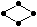
\includegraphics[scale=2.5]{desenhos/ciclo.png}
\end{center}

Veja que não desenhamos uma aresta ligando $a$ e $d$, pois o desenho já mostra que $a<b$ e $b<d$.

    \item Um exemplo um pouco maior
    
    \begin{center}
        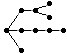
\includegraphics[scale=2.5]{desenhos/arvre.png}
\end{center}


\item Também podemos ter ordens infinitas. A ordem dos números inteiros, por exemplo, é dada por

    \begin{center}
        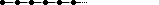
\includegraphics[scale=2.5]{desenhos/zsemcordirec.png}
\end{center}




  \end{itemize}



\end{exemplo*}

Nosso paradigma de número que queremos emular é o dos número naturais: começamos com o $0$, e depois vem o $1$, e depois vem o $2$, e assim por diante. O que essa ordem tem de especial? Primeiramente, ela é total, o que já a diferencia, por exemplo, dos nossos dois primeiros exemplos. Já a ordem do terceiro exemplo é total, mas ela falta um começo, ou seja, um menor elemento. Poderiamos artificialmente colocar um menor elemento nessa ordem, mas ainda assim tem algo ali faltando: o menor elemento não tem um único sucessor, isto é, um único elemento que vem depois dele e é menor que todos os outros que vem depois. Ok, uma ordem total com sucessor pra todo elemento é o que queremos?

\begin{exercicio}
\luafacil Dê exemplo de uma ordem total, com menor elemento, que todos os elementos possuem sucessor, mas que existe uma sequência decrescente infinita.
\end{exercicio}

Sequências decrescentes infinitas não existem nos naturais. Vamos nomear esta propriedade.

\begin{definicao*}[Boa fundação]
  Uma ordem em um conjunto $A$ é bem fundada se pra todo subconjunto $B \subset A$ não vazio, existe um elemento $b \in B$ que não é maior que nenhum outro elemento de $B$, dito um elemento minimal.
\end{definicao*}

\begin{exercicio}
  \luafacil Mostre que a definição dada de boa fundação é equivalente a não existência de sequências decrescentes infinitas.
\end{exercicio}

Juntando este pedido com o pedido de totalidade da ordem, chegamos a nossa definição principal.

\begin{definicao*}[Boa ordem]
  Uma boa ordem em um conjunto $A$ é uma ordem total e bem fundada.
\end{definicao*}

Um detalhe aqui é que na definição de boa fundação, pedimos apenas a existência de um elemento minimal no $B$, não necessariamente um mínimo de $B$, que seria um elemento explicitamente menor que todos os outros. Como em uma boa ordem estamos pedindo também totalidade da ordem, o elemento minimal do $B$ será também um mínimo.

Um bom indicativo de que estamos indo na direção correta é que de posse da propriedade de boa fundação, já conseguimos generalizar uma das propriedades mais caracterizadoras dos números naturais: o princípio de indução.

\begin{teorema*}[Indução sobre uma ordem bem fundada]
Seja $A$ um conjunto com uma ordem bem fundada. Dado um $x \in A$, defina $\text{Antes}_x \defeq \{y \in A \mid y < x \}$. Suponha que $B \subset A$ é tal que satisfaz o princípio indutivo:
\[
\text{Antes}_x \subset B \implies x \in B
\]

Então $B = A$
\end{teorema*}
\begin{prova}
Suponha que $A \setminus B$ seja não vazio. Então, ele possui um menor elemento $m \in A \setminus B$. Daí $\text{Antes}_m$ deve estar contido no complementar de $A \setminus B$, ou seja, em $B$. Pelo princípio indutivo, temos $m \in B$, contradição.
\end{prova}

Vamos construir um entendimento melhor de quem são essas boas ordens.

\begin{exemplo*}[As primeiras  boas ordens]
  Qualquer ordem dada por um caminho finito

    \begin{center}
        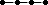
\includegraphics[scale=2.5]{desenhos/caminho finito.png}
\end{center}

  é uma boa ordem, a usual dada por uma quantidade finita de números naturais, como $1<2<3<4$. Se quisermos todos os números naturais, fazemos um caminho infinito

    \begin{center}
        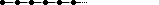
\includegraphics[scale=2.5]{desenhos/caminho infinito.png}
\end{center}

onde cada vértice é menor o que todos que o seguem.

E se colocarmos um vértice a mais, ``na frente'' de todos estes, simbolizando que temos um elemento maior que todos estes?

    \begin{center}
        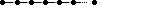
\includegraphics[scale=2.5]{desenhos/omega.png}
\end{center}

Continuamos tendo uma boa ordem. E poderiamos ter seguido, com mais um vértice a frente do outro

    \begin{center}
        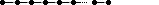
\includegraphics[scale=2.5]{desenhos/omegamaisum.png}
\end{center}

e mais um

    \begin{center}
        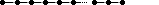
\includegraphics[scale=2.5]{desenhos/omegamaisdois.png}
\end{center}

e mais infinitos

    \begin{center}
        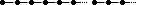
\includegraphics[scale=2.5]{desenhos/omegamaisomega.png}
\end{center}

e mais um depois desses infinitos

    \begin{center}
        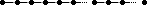
\includegraphics[scale=2.5]{desenhos/omegamaisomegamaisum.png}
\end{center}

E assim por diante...


    \begin{center}
        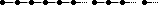
\includegraphics[scale=2.5]{desenhos/omegamaisomegamaisomega.png}
\end{center}

\end{exemplo*}

Veja como as construções deste exemplo funcionaram: sempre que chegamos em um elemento final, adicionamos um elemento a mais após ele. E se fizermos isso infinitas vezes, obtendo uma sequência crescente infinita, adicionamos um elemento maior que todos esses. E se repetirmos esse processo infinitas vezes, adicionamos ainda mais um elemento que vem depois disso tudo. Qualquer boa ordem vai ser essencialmente a mesma (isomorfa) a uma ordem construida (mais ou menos) dessa forma. Nosso trabalho agora é formalizar essa construção, para que possamos ter uma visão clara destas boa ordens, que serão os nossos buscados ordinais.


\begin{definicao*}[Ordinais]
  Um ordinal é um conjunto $\alpha$ que satisfaz
  
  \begin{itemize}[label=\ding{212}]
    \item se $\beta \in \alpha$ e $\gamma \in \beta$, então $\gamma \in \alpha$ (conjunto transitivo)
    \item a relação de pertencimento $\in$ entre os elementos de $\alpha$ é uma boa ordem
  \end{itemize}
\end{definicao*}

Não se assuste com a definição. Vamos tentar te convencer que ela captura concisamente os exemplos desenhados anteriormente, dando para gente um objeto canônico para cada classe de conjuntos bem ordenados, e generalizando a ordem dos números naturais para além dos objetos finitos.

A origem dessa definição vem de capturar a seguinte construção, que é a forma canônica de implementar os números naturais como conjuntos na axiomática ZFC. Começamos definindo $0 \defeq \varnothing$. Formamos o $1$ coletando $0$ em um conjunto $1 \defeq \{\varnothing\}$. Formamos o $2$ coletando todos os anteriores $2 \defeq \{0,1\} = \{\varnothing, \{\varnothing\}\}$. Seguimos assim, ou seja, iterando a operação $S(\alpha) \defeq \alpha \cup \{\alpha\}$.
\begin{align*}
3 &\defeq S(2) = 2 \cup \{2\} =  \{0,1,2\} \\
4 &\defeq S(3) = 3 \cup \{3\} = \{0,1,2,3\}
\end{align*}

Os conjuntos construídos iterando essa operação finitas vezes são todos transitivos. Além disso, a relação de pertencimento $\in$ funciona como a ordem dos naturais: $0 \in 1 \in 2 \in 3 \in \dots$, pois $\alpha \in S(\alpha)$. Assim, $\in$ é uma ordem total em cada um desses $\alpha$. Para vermos que é uma boa ordem, resta apenas mostrar a boa fundação, que é a existência de menor elemento em todo subconjunto, ou, equivalentemente, a não existência de sequências decrescentes infinitas. É claro que aqui isto é óbvio pelos conjuntos serem finitos, mas já podemos mencionar aqui que no caso geral não precisamos nos preocupar em provar que $\in$ é bem fundado, pois isto é já é um dos axiomas de ZFC.

\begin{exercicio}
  \luamedio Cheque o que o Axioma da Fundação diz e o use para provar que não existe conjunto $A$ tal que $A \in A$ e que não existe sequência infinita $A_i$ de conjuntos tal que $A_{i+1} \in A_i$ para todo $i \in \mathbb{N}$. (Dica: use construções usuais de conjuntos e se quiser ser formal, explicite os axiomas necessários para estas construções). Se convença que isso é suficiente para garantir que se $\in$ define uma ordem total em um conjunto $A$ então esta ordem é uma boa ordem.
\end{exercicio}

Temos então já uma classe de ordinais, que vamos chamar de ordinais finitos, ou de números naturais. Construimos estes começando a partir de um elemento minimal, o $0$ e iterando uma operação de sucessão, $S(\alpha)$, assim como na construção dos exemplos anteriores. Qual é o análogo da operação de adicionar um elemento ao infinito após uma sequência infinita de sucessões? Bom, se estavamos definindo um número como o conjunto de todos os seus antecessores, então poderiamos definir $\omega$ como o conjunto de todos os números naturais. $\omega$ é claramente transitivo, e como $\in$ ordena os naturais na sua ordem usual, temos uma ordem total e portanto uma boa ordem. Assim, $\omega$ é um ordinal tal que qualquer número natural $n \in \omega$. Com ele, podemos iterar sucessores novamente...

\begin{align*}
  \omega + 1 &\defeq S(\omega) = \omega \cup \{\omega\} \\
  \omega + 2 &\defeq S(\omega + 1) \\
  \omega + 3 &\defeq S(\omega + 2)
\end{align*}

E é claro, $\omega \in \omega + 1 \in \omega + 2 \in \omega + 3 \in \dots$. Unindo todos estes $\omega + n$ criamos um novo ordinal, conhecido como $\omega 2$. E aí fazemos o $S(\omega 2)$ ...

O que está acontecendo aqui é que a relação de pertencimento ultimamente codifica a ordem que estamos buscando. A operação de sucessão de um ordinal captura a ideia de criar um elemento logo após este ordinal, e a união de uma coleção infinita de ordinais cria um novo ordinal após todos eles. 

Vamos botar todas essas ideias em um único teorema.

\begin{teorema*}[$\in$ ordena totalmente os ordinais e operações de sucessão e limite]
  Seja $\alpha$ um ordinal e $A$ um conjunto de ordinais.
  \begin{itemize}[label = \ding{212}]
  \item Se $\beta$ é algum outro ordinal distinto de $\alpha$, então ou $\alpha \in \beta$ ou $\beta \in \alpha$. Além disso, qualquer outro elemento $\gamma \in \alpha$ é também um ordinal.
  \item $S(\alpha) \defeq \alpha \cup \{\alpha\}$ é um ordinal tal que $\alpha \in S(\alpha)$ e não existe nenhum outro ordinal $\beta$ tal que $\alpha \in \beta \in S(\alpha)$
  \item  $L(A) \defeq \underset{\alpha \in A}{\bigcup} \alpha = \{\gamma \mid \gamma \in \alpha \in A\}$ é um ordinal. Se $A$ possui um elemento $\beta$ tal que $\gamma \in \beta$ para todo $\gamma \in A$ (ou seja, um maior elemento), então $L(A) = \beta$. 
  
  Caso contrário, $L(A)$ é um ordinal distinto de todos em $A$ que satisfaz $\gamma \in L(A)$ para todo $\gamma \in A$. Ele é o menor com essa propriedade: se existe um ordinal $\beta$ tal que $\gamma \in \beta$ para todo $\gamma \in A$, então $L(A) \in \beta$.
  \end{itemize}
\end{teorema*}
\begin{prova}
  Vamos por partes.
  \begin{itemize}[label = \ding{212}]
    \item  Tome $\beta$ ordinal distinto de $\alpha$ e considere a interseção $I = \alpha \cap \beta$. Note que $I$ é transitivo. Como $I \subset \alpha$, podemos considerar o subconjunto $\alpha \setminus I$ de $\alpha$. Se ele for não vazio, então deverá ter um menor elemento (em relação a $\in$), que chamamos de $i$. Agora, veja que $i \subset I$, pois se um elemento $a \in i$ não estivesse em $I$, ele estaria em $\alpha \setminus I$, mas pela minimalidade de $i$ teriamos $i \in a$, o que fecharia um loop $ a \in i \in a$, proibido pelo Axioma da Fundação. Mas também conseguimos provar $I \subset i$, pois um elemento $a \in I$ deve satisfazer $a \in i$ ou $i \in a$, por $\alpha$ ser totalmente ordenado por $\in$. Mas $i \in a$ implicaria $i \in I$ pela transitividade de $I$, e isto contradiz $i \in \alpha \setminus I$. Concluimos que $i = I$, e assim a própria interseção $I$ é um elemento de $\alpha$.
    
    Da mesma forma, se $\beta \setminus I$ for não vazio, conseguimos mostrar que $I \in \beta$. Assim, não podemos ter ao mesmo tempo $\alpha \setminus I$ e $\beta \setminus I$ não vazios, pois nesse caso teriamos $I \in \alpha$ e $I \in \beta$, ou seja, $I \in \alpha \cap \b = I$, contradizendo o Axioma da Fundação.

    Digamos então que o $\beta \setminus I$ é vazio e $\alpha \setminus I$ é não vazio. Nesse caso, temos que $\beta \subset \alpha$, ou seja $I = \beta$. Como acabamos de mostrar, $\alpha \setminus I$ ser não vazio implica que $I \in \alpha$, e logo $\beta = I \in \alpha$. E é claro, o outro caso $\alpha \setminus I$ vazio vai levar a conclusão que $\alpha \in \beta$.

    \item $S(\alpha)$ ser um ordinal é imediato de $\alpha$ ser um ordinal: tome $\gamma \in \beta \in S(\alpha)$. Se $\beta = \alpha$, então $\gamma \in \alpha \subset S(\alpha)$, logo $\gamma \in S(\alpha)$. Se $\beta \in \alpha$, então $\gamma \in \alpha$ por transitividade de $\alpha$, logo $\gamma \in S(\alpha)$. Isso mostra a transitividade de $S(\alpha)$. Para mostrar que $S(\alpha)$ é totalmente ordenado, veja que todos os pares de elementos dentro de $\alpha$ já são comparáveis pois $\alpha$ é totalmente ordenado. O único outro possível par é um elemento $\beta \in \alpha$ com o próprio $\alpha$, que já satisfazem uma relação de pertencimento e portanto são comparáveis. Isto mostra que $S(\alpha)$ é ordinal.
    
    Agora, $\alpha \in S(\alpha)$ por definição. Se existisse um $\beta$ tal que $\alpha \in \beta \in S(\alpha)$ teriamos ou $\beta = \alpha$ ou $\beta \in \alpha$, ambos contradizendo o Axioma da Fundação.
    
    \item Todas as propriedades de $L(A)$ seguem diretamente usando métodos similares aos do item anterior, então, deixamos como exercício.
  \end{itemize}
\end{prova}

\begin{exercicio}
  \luafacil Finalize a demonstração do teorema anterior com as provas das propriedades de $L(A)$.
\end{exercicio}

Veja que pelo primeiro ponto do teorema, $\in$ define uma ordem total nos ordinais, e, de fato, pelo Axioma da Fundação, $\in$ é bem fundado e logo $\in$ define uma boa ordem nos ordinais... Mais ou menos. Ingenuamente até agora estamos coletando ordinais em conjuntos sem nos preocupar, mas se tentarmos criar um conjunto de todos os ordinais, vamos cair em problemas.

\begin{exercicio}
  \luamedio Encontre uma contradição se supormos que existe um conjunto de todos os ordinais.
\end{exercicio}

Vamos fingir que não vimos isso e seguirmos nossa vida. 

A partir de agora, falamos de ordinais serem maiores ou menores que outros, escrevendo $\alpha < \beta$, sempre querendo dizer que $\alpha \in \beta$. Também vamos escrever $S(\alpha) = \alpha + 1$, como vai ser justificado mais tarde com a introdução da aritmética ordinal.

Dado um ordinal qualquer $\alpha$, temos que ou $\varnothing \in \alpha$ ou $\alpha \in \varnothing$ pelo primeiro ponto do toerema anterior. Mas $\varnothing$ não possui elementos, logo $\varnothing \in \alpha$. Assim, $\varnothing$, que definimos anteriormente como o $0$ é o menor ordinal. Pelo segundo ponto, $1 = S(0)$ é o próximo ordinal, sem nenhum entre eles. Seguindo assim, vemos que as construções que fizemos dos números naturais e após estes o $\omega$, os $\omega + n$ e por aí em diante formam exatamente o início dos ordinais.

Uma forma melhor de visualizar é este processo é, ao invés de colocarmos os elementos em uma sequência linear, os colocamos em círculos. E toda vez que colocamos um novo elemento sucessor, diminuimos a distância do anterior de forma que as distâncias entre eles formam uma série convergente. Assim, o passo limite é realmente um limite de uma sequência convergente. Seguimos assim, usando convergências para visualizar os passos limites, diminuindo os passos e o raio do círculo, formando uma espiral:

(espiral)

O maior uso que vamos ter para ordinais nesse livro é através da generalização do princípio de indução sobre os naturais para um princípio de indução sobre os ordinais, conhecida como indução transfinita. Muitos objetos de tamanhos arbitrariamente grandes podem ser construidos passo-a-passo, mas possivelmente com mais de uma infinitude de passos. A indução transfinita consegue alcançar estes objetos.

Já mostramos mais cedo que indução sobre uma boa ordem funciona. Vamos simplesmente adaptar aquele teorema pra sua versão ordinal.

\begin{teorema*}[Indução transfinita]
  Seja $P(\alpha)$ alguma propriedade que pode ser ou verdadeira ou falsa para um dado ordinal $\alpha$. Suponha que valha o princípio indutivo

  \[ \forall \beta < \alpha P(\beta)  \implies P(\alpha) \]

  Então $P(\alpha)$ vale para todo $\alpha$.
\end{teorema*}
\begin{prova}
  Se a classe de todos os ordinais fosse um conjunto, poderiamos simplesmente usar o teorema de indução sobre uma boa ordem neste conjunto. Como não podemos fazer isso, aplicamos o teorema num conjunto menor. Tome $\alpha$ um ordinal. Sabemos que seu sucessor $\alpha + 1$ é bem ordenado pela relação de pertencimento usual dos ordinais. Considere $B = \{ \beta \in \alpha + 1 \mid P(\beta)\}) \subset \alpha + 1$. O princípio indutivo vai valer em $B$, logo pelo teorema de indução sobre uma boa ordem podemos concluir que $B = \alpha + 1$. Como $\alpha \in \alpha + 1$, concluimos que vale $P(\alpha)$.
\end{prova}

Na indução para os naturais, geralmente dividimos a demonstração em duas partes: provar o caso base, que tende a ser $P(0)$, e provar que $P(n)$ segue de $P(m)$ para $m<n$. Análogamente, no caso infinito, geralmente dividimos a demonstração em duas partes. Provamos o princípio indutivo para o caso onde o ordinal é sucessor de algum outro ordinal, e depois provamos para quando ele não é sucessor de ninguém. Estes dois tipos de ordinais são distintos o suficientes para merecerem nomes.

\begin{definicao*}[Ordinal sucessor e ordinal limite]
  Um ordinal $\alpha$ é dito sucessor se $\alpha = \beta + 1$ para algum outro ordinal $\beta$. Caso contrário, o ordinal é dito um ordinal limite.
\end{definicao*}

Veja que quando $\alpha$ é um ordinal limite, ele é exatamente o limite de todos os seus ordinais anteriores $\alpha = L(\{\beta \mid \beta < \alpha\})$ como na nossa definição anterior de limite.

Mencionamos mais cedo a afirmação ousada de que os ordinais exaustam todas as possíveis boa ordens. É claro, ``ser a mesma ordem'' é uma noção capturada pelo isomorfismo apropriado da categoria que estamos trabalhando.

\begin{definicao*}[Isomorfismo de ordens]
Duas ordens $A,B$ são isomorfas se existe uma bijeção $f:A \rightarrow B$ tal que $f(a) < f(b)$ se e somente se $a < b$.
\end{definicao*}

\begin{teorema*}[Ordinais são representantes de boa ordens]
  Todo conjunto bem ordenado $A$ é isomorfo a um único ordinal $\alpha$.
\end{teorema*}
\begin{prova}
Vamos esboçar a demonstração.

Por indução transfinita, conseguimos provar que nenhum ordinal é isomorfo entre si, e assim temos a parte da unicidade.

Tome um $a \in A$. Se existir algum ordinal $\alpha$ tal que $\text{Antes}_a$ é isomorfo a $\alpha$, chame o $a$ de um elemento bom e defina $f(a) = \alpha$. Considere $B$ o subconjunto de $A$ dos elementos que não são bons. Se $B$ for não vazio, então como $A$ é bem ordenado, $B$ deveria ter menor elemento, digamos $b$. Assim, todo elemento de $\text{Antes}_b$ é bom. Agora bastaria tomar o menor ordinal maior que os ordinais associados aos elementos de $\text{Antes}_b$ e teriamos um ordinal isomorfo a $\text{Antes}_b$, contradizendo $b$ não ser bom. Concluimos que $B$ é vazio. Agora fazemos o mesmo truque de tomar o menor ordinal $\gamma$ maior que todos os $f(a)$ para cada $a \in A$, e este será o tal que $\gamma \cong A$.
\end{prova}

\begin{exercicio}
  \luamedio Complete os detalhes da demonstração anterior. Se já estudou a axiomática, procure onde está escondido um uso do Axioma da Substituição.
\end{exercicio}

Conhecendo este teorema, você poderia ter se perguntando porque não definimos um ordinal simplesmente como uma classe de equivalência de boas ordens. Minha primeira vez ouvindo sobre ordinais foi exatamente assim: tome a categoria de boa ordens, e a quociente por isomorfismo de ordem - o que resta é a categoria dos ordinais. O único problema disso é que esta suposta classe de equivalência não é um objeto de ZFC, isto é, não é um conjunto. Essa dificuldade formal nos leva a busca pela construção de uma boa ordem canônica pra se escolher em cada classe de equivalência, dando origem a nossa definição apresentada dos ordinais.

Pra finalizar nossa introdução aos ordinais, vamos justificar porque nomeamos ordinais como $\omega + 1$, $\omega + 3$ e $\omega 2$. Estes nomes não são arbitrários: eles representam operações aritméticas bem definidas sobre os ordinais, que nos permitem contemplar mais e mais ordinais.

Sejam $\alpha,\beta$ dois ordinais. A ideia é simples: queremos que $\alpha + \beta$ seja o ordinal referente a ordem dada quando colocamos a ordem do $\beta$ logo a frente da ordem do $\alpha$. Para formalizarmos isto, defina o conjunto $S = \alpha \times \{0\} \cup \beta \times \{1\}$. Defina uma ordem sobre $S$ colocando $(a,0) < (a',0)$ sempre que $a<a'$ em $\alpha$ e $(b,1) < (b',1)$ sempre que $b<b'$, e também que $(a,0) < (b,1)$ para quaisquer $a \in \alpha$ e $b \in \beta$.

\begin{exercicio}
  \luafacil Mostre que isto define uma boa ordem em $S$.
\end{exercicio}

\begin{definicao*}[Soma de ordinais]
   Dados dois ordinais $\alpha,\beta$, a soma $\alpha + \beta$ será o o único ordinal isomorfo a boa ordem de $S$ descrita no parágrafo anterior.
\end{definicao*}

\begin{exercicio}
  \luafacil Se convença que $\alpha + 1$ segundo nossa definição de adição é exatamente o sucessor de $\alpha$.
\end{exercicio}

\begin{exercicio}
\luafacil Mostre que $1 + \omega = \omega$ e conclua que esta soma não é comutativa.
\end{exercicio}

A intuição da soma é que estamos concatenando as ordens. E se agora quisermos concatenar uma mesma ordem $\alpha$ uma quantidade $\beta$ de vezes? Ou seja, estamos iterando a soma: estamos multiplicando.

Dados dois ordinais $\alpha,\beta$, defina $P = \beta \times \alpha$ (sim, nesta ordem mesmo). Definimos em $P$ a ordem lexicográfica - aquela famosa por dicionários. Colocamos $(b,a) < (b',a')$ sempre que $b < b'$. E quando o par tiver o mesmo elemento na sua primeira coordenada, a segunda coordenada decide a ordem: $(b,a) < (b,a')$ se $a < a'$.

\begin{exercicio}
  \luafacil Mostre que isto define uma boa ordem em $P$.
\end{exercicio}

\begin{definicao*}[Produto de ordinais]
Dados dois ordinais $\alpha,\beta$, seu produto $\alpha \beta$ será o único ordinal isomorfo a boa ordem de $P$ descrita no parágrafo anterior.
\end{definicao*}

\begin{exercicio}
  \luafacil Mostre que $\alpha 1 = \alpha$ e $\alpha 2 = \alpha + \alpha$.
\end{exercicio}

\begin{exercicio}
  \luafacil Mostre que $2 \omega = \omega$ e conclua que este produto não é comutativo.
\end{exercicio}

Com estas operações, o começo dos ordinais se torna fácil de nomear. Começamos com $0,1,2,\dots, \omega, \omega + 1, \omega + 2, \omega +3, \dots, \omega + \omega = \omega 2, \omega2 + 1, \omega2 + 2, \dots, \omega2 + \omega = \omega 3, \omega 3 + 1, \omega 3 + 2, \dots$. Continuando assim, obtemos $\omega 3, \omega 4, \omega 5, \dots$, e o limite desta sequência agora é $\omega \omega$. Não faria sentido esse ordinal ser $\omega ^ 2$? Vamos definir exponenciação.

Uma outra forma de se pensar a adição $\alpha + \beta$ é pensar que estamos iterando $\beta$ vezes a operação de sucessor no $\alpha$. Da mesma forma, a multiplicação $\alpha \beta$ se dá pela soma de $\alpha$ com ele mesmo $\beta$ vezes. Exponenciação é a continuação natural: e se quisermos definir $\alpha^{\beta}$ como sendo $\beta$ vezes o produto de $\alpha$ por ele mesmo? Ainda podemos fazer esta definição explicitamente como fizemos nos casos anteriores, mas para ilustrar um método diferentem, vamos definir a exponenciação por indução, assim como poderiamos ter feito no caso da adição ou multiplicação. Dado dois ordinais $\alpha,\beta$, faremos a indução no $\beta$, ou seja, supomos que $\alpha^{\gamma}$ já está bem definido para todo $\gamma < \beta$, e com isso definimos o $\alpha^\beta$. Para formalizar esta construção, precisariamos provar um teorema sobre construções recursivas, que é inteiramente análogo ao teorema de indução sobre ordinais que já apresentamos, então omitimos apelando para a intuição e boa vontade da leitora.

\begin{definicao*}[Exponenciação de ordinais]
  Sejam $\alpha,\beta$ ordinais. Se $\beta = 0$, defina $\alpha^0 = 1$. Suponha $\alpha^\gamma$ já bem definido para todo $\gamma < \beta$. Então, defina
  \begin{itemize}[label=\ding{212}]
    \item $\alpha^{\beta} = \alpha \alpha^{\gamma}$ se $\beta$ é ordinal sucessor e $\beta = \gamma + 1$
    \item $\alpha^{\beta} = L(\{\alpha^{\gamma} \mid \gamma < \beta\})$ se $\beta$ é ordinal limite
  \end{itemize}

\end{definicao*}

\begin{exercicio}
  \luamedio Encontre definições indutivas para adição e para a multiplicação similares a da exponenciação.
\end{exercicio}

Assim, agora podemos continuar nossa lista de ordinais, passando do $\omega \omega = \omega ^ {2}$ para o $\omega^{3}$ e assim por diante.Tomando o limite dos $\omega, \omega^2, \omega^3, \omega^4, \dots$, chegamos ao $\omega ^\omega$. 

\begin{exercicio}
  \luafacil Contemple o caminho do $\omega^\omega$ até o $\omega^{\omega^{\omega}}$.
\end{exercicio}

E o $\omega^{\omega^{\omega^{\omega}}}$? Podemos continuar este jogo infantil de criar números maiores e maiores, operações iteradas de operações iteradas. Conseguimos criar ordinais como $\epsilon_0$, que é o limite dos $\omega, \omega^\omega, \omega^{\omega^{\omega}}, \dots$ e satisfaz a propriedade surpreendente que $\epsilon_0 = \omega^{\epsilon_0}$. Os ordinais que vem antes do $\epsilon_0$ podem ser descritos com a chamada forma normal de Cantor, que é essencialmente uma expansão na base $\omega$ do ordinal: $\alpha = \omega^{\beta_1}c_1 + \omega^{\beta_2}c_2 + \dots + \omega^{\beta_n}c_n$, onde $\beta_i$ são ordinais e $c_i$ são números naturais. Na verdade, ordinais depois dos $\epsilon_0$ também admitem esta escrita, mas ela não simplifica a nossa descrição do ordinal. Veja, o próprio $\epsilon_0$ tem como forma normal $\epsilon_0 = \omega^{\epsilon_0}$ - o expoente que aparece no $\omega$ é o próprio ordinal! Para todos os ordinais antes do $\epsilon_0$, os expoentes $\beta_i$ são estritamente menores que o ordinal.

A minha propriedade favorita do $\epsilon_0$ é que ele ainda é contável. Não chegamos nem perto do primeiro ordinal incontável, $\omega_1$. Mas estou me adiantando. Agora que aprendemos a colocar coisas atrás de outras coisas, vamos voltar pro chão e aprender a contar.

\section{Aprendendo a contar}




\end{document}
